\documentclass[12pt]{article}
\usepackage[left=2cm,right=2cm,top=2cm,bottom=2cm,bindingoffset=0cm]{geometry}
\usepackage[utf8x]{inputenc}
\usepackage[english,russian]{babel}
\usepackage{cmap}
\usepackage{graphicx}
\usepackage{amssymb}
\usepackage{amsmath}
\usepackage{ bbold }
\usepackage{url}
\usepackage{pifont}
\usepackage{tikz}
\usepackage{verbatim}
\usepackage[most]{tcolorbox}

\newcommand{\R}{\mathbb{R}} % set of real numbers
\renewcommand{\inf}{\infty}
\newcommand{\la}{\lambda}

\definecolor{block-gray}{gray}{0.90} 
\newtcolorbox{myquote}{colback=block-gray,grow to right by=-10mm,grow to left by=-10mm,
boxrule=0pt,boxsep=0pt,breakable} 




\begin{document}
\begin{center} {\LARGE Формальные языки. Задание на зачёт} \end{center}

\bigskip

 Правила грамматики: 
\begin{myquote}
\begin{enumerate}
\item $S \to aBcd$
\item $S \to aFcg$
\item $B \to aBc$
\item $B \to b$
\item $F \to aFc$
\item $F \to f$
\end{enumerate}
\end{myquote}
Корректность: из стартового нетерминала выбираем тип цепочки -- с $f/g$ или $b/d$, и наращиваем вместе $a$-шки и $b$-шки, причём хотя бы одна такая пара есть.\\

Построим автомат:\\

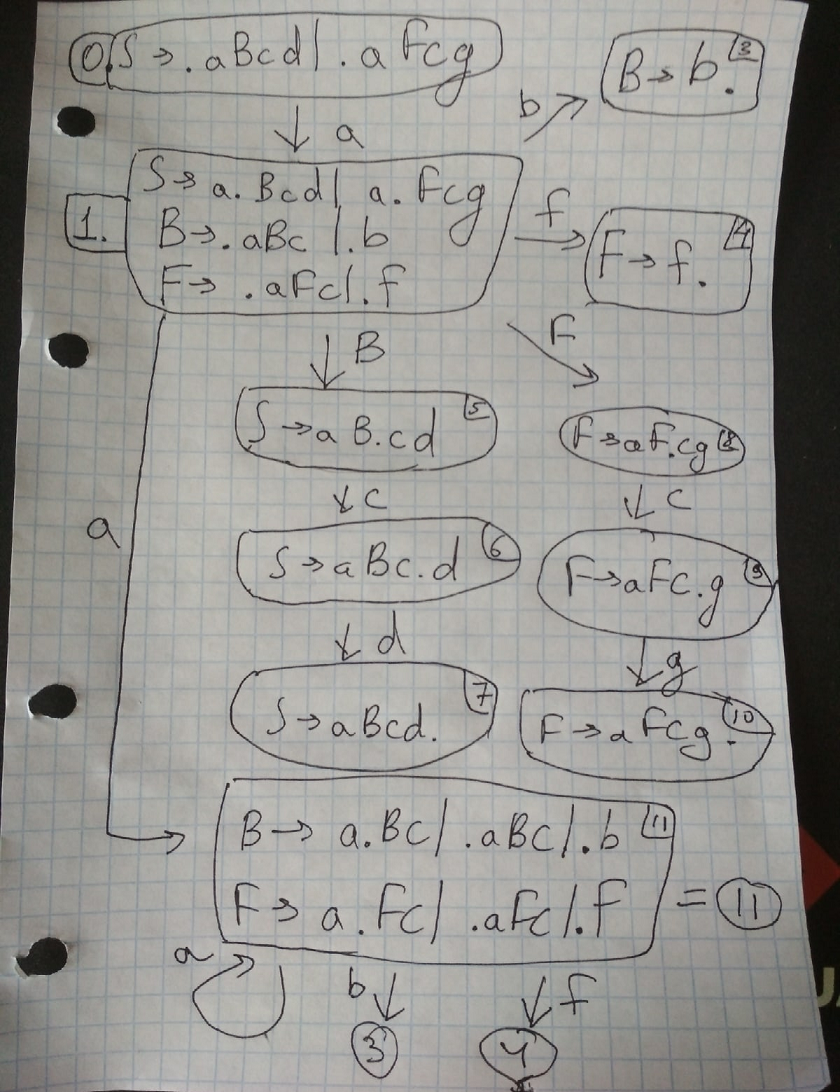
\includegraphics{automaton1}
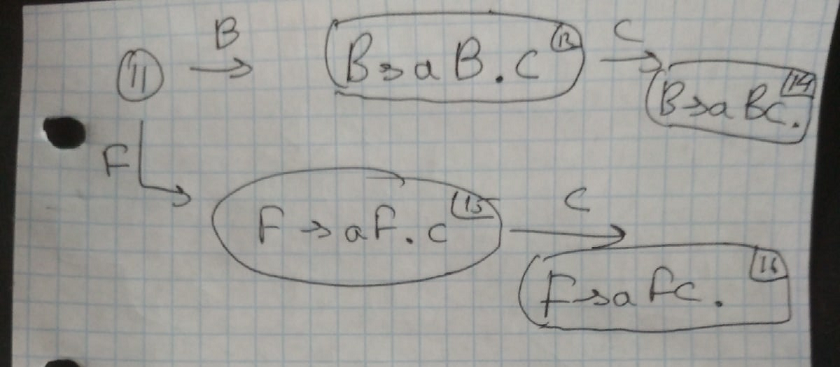
\includegraphics{automaton2}
(там описка в айтемах 8, 9 и 10 слева нетерминал $S$. А ещё 2 и 12 айтема не существует в природе)\\

Множества FOLLOW для нетерминалов: \\
\begin{tabular}{ | l | l | }
\hline
$S$ & $\{\$\}$\\ \hline
$B$ & $\{c\}$\\ \hline
$F$ & $\{c\}$\\ 
\hline
\end{tabular}\\


SLR-таблица:\\
\begin{tabular}{| l || l | l | l | l | l | l | l || l | l |}
\hline
item &  $a$ & $b$ & $c$ & $d$ & $f$ & $g$ & $\$$ & $B$ & $F$ \\ \hline
0 &  $s_1$ & $$ & $$ & $$ & $$ & $$ & $$ &  $$ & $$ \\ \hline
1 &  $s_{11}$ & $s_3$ & $$ & $$ & $s_4$ & $$ & $$ & $5$ & $8$ \\ \hline
3 &  $$ & $$ & $r_4$ & $$ & $$ &  $$ & $$ & $$ & $$ \\ \hline
4 &  $$ & $$ & $r_6$ & $$ & $$ &  $$ & $$ & $$ & $$\\ \hline
5 &  $$ & $$ & $s_6$ & $$ & $$ &  $$ & $$ & $$ & $$\\ \hline
6 &  $$ & $$ & $$ & $s_7$ & $$ &  $$ & $$ & $$ & $$\\ \hline
7 &  $$ & $$ & $$ & $$ & $$ &  $$ & acc & $$ & $$\\ \hline
8 &  $$ & $$ & $s_9$ & $$ & $$ &  $$ & $$ & $$ & $$\\ \hline
9 &  $$ & $$ & $$ & $$ & $$ &  $s_{10}$ & $$ & $$ & $$\\ \hline
10 &  $$ & $$ & $$ & $$ & $$ &  $$ & acc & $$ & $$\\ \hline
11 &  $s_{11}$ & $s_3$ & $$ & $$ & $s_4$ & $$ & $$ & $13$ & $15$ \\ \hline
13 &  & & $s_{14}$ & & &  & & & \\ \hline 
14 & & & $r_3$ & & & & & &\\ \hline
15 &  & & $s_{16}$ & & &  & & & \\ \hline 
16 & & & $r_5$ & & & & & &\\ \hline
\end{tabular}
\newpage
Пример разборов строк.\\

aaabcccd:\\

\begin{tabular}{| l | | l | | l |}
\hline
строка & стек & инструкция \\ \hline
aaabcccd\$ & 0 & $s_1$ \\ \hline
aabcccd\$ & 0 a 1 & $s_{11}$ \\ \hline
abcccd\$ & 0 a 1 a 11 & $s_{11}$ \\ \hline
bcccd\$ & 0 a 1 a 11 a 11 & $s_3$ \\ \hline 
cccd\$ & 0 a 1 a 11 a 11 b 3 & $r_4$  \\ \hline
cccd\$ & 0 a 1 a 11 a 11 B 13 & $s_{14}$ \\ \hline
ccd\$ & 0 a 1 a 11 a 11 B 13 c 14 & $r_{3}$ \\ \hline
ccd\$ & 0 a 1 a 11 B 13 & $s_{14}$ \\ \hline
cd\$ & 0 a 1 a 11 B 13 c 14 & $r_{3}$ \\ \hline
cd\$ & 0 a 1 B 5 & $s_6$ \\ \hline
d\$ & 0 a 1 B 5 c 6 & $s_7$ \\ \hline
\$ &0 a 1 B 5 c 6 d 7 & acc \\ \hline
& 0 & стек пустой, acc, всё ок \\ \hline
\end{tabular}\\

aaaafcg:\\

\begin{tabular}{| l | | l | | l |}
\hline
строка & стек & инструкция \\ \hline
aaaafcg\$ & 0 & $s_1$ \\ \hline
aaafcg\$ & 0 a 1 & $s_{11}$ \\ \hline
aafcg\$ & 0 a 1 a 11 & $s_{11}$ \\ \hline
afcg\$ & 0 a 1 a 11 a 11 & $s_{11}$ \\ \hline
fcg\$ & 0 a 1 a 11 a 11 a 11 & $s_{4}$ \\ \hline
cg\$ & 0 a 1 a 11 a 11 a 11 f 4 & $r_{6}$ \\ \hline
cg\$ &0 a 1 a 11 a 11 a 11 F 15 & $s_{16}$ \\ \hline
g\$ &0 a 1 a 11 a 11 a 11 F 15 c 16 & $r_{5}$ \\ \hline
g\$ &0 a 1 a 11 a 11 F 15 & fail \\ \hline
\end{tabular}

\end{document}
